%!TEX program = xelatex
%!TEX TS-program = xelatex
%!TEX encoding = UTF-8 Unicode

\documentclass[10pt]{article}
\usepackage{url}
\usepackage{fontspec,xltxtra,xunicode}
\usepackage[colorlinks,linkcolor=blue]{hyperref}
\usepackage{graphicx}

\defaultfontfeatures{Mapping=tex-text}
\setromanfont{Songti SC}
\XeTeXlinebreaklocale "zh"
\XeTeXlinebreakskip = 0pt plus 1pt minus 0.1pt
\author{陈根宝}
\title{TDM 离线训练升级合作}
\date{}
\newfontfamily{\H}{Songti SC}
\newfontfamily{\E}{Weibei SC}
\begin{document}
\maketitle
\section{背景}
基于树的深度检索方案在广告推荐领域被证明是有效的,具体参见\href{https://www.atatech.org/articles/102403}{ATA文章}。
但是这种方案对树的构建及初始化有着比较重度的依赖,特别是当系统超过一定规模时候,
这种树结构可能不能在单机上存储,从而使整个技术方案面临挑战。本文旨在提出一种高效的分布式
树构建及存储方案,作为整个TDM训练(未来可能涉及在线检索)方案的基石。

\section{需求}
根据 TDM 技术实现细节,TDM的主要训练过程为: 初始树 -> 模型训练 -> 树重建 -> 模型再训练的循环迭代过程以及模型评测过程,
梳理训练及评测过程中的具体操作我们发现对树的功能需求主要有以下几个:
\begin{enumerate}
\item 初始化: 把所有的item按类目排序,然后直接递归地分类来构建分类树。
\item 树重建:通过item embedding逐层kmeans聚类的方式,最终形成一颗多层的分类树。
\item 高效存取、序列化: 整棵树需要支持序列化以支持在不同阶段存取,同时在训练过程中会高频地进行结点的存取,
  比如在采样过程中会同时选取批量结点进行打分排序,因此树结点的高效存取对整个训练过程的效率至关重要。
\item 策略化采样: 采样是整个训练过程非常重要的一环,支持灵活可扩展的采样策略会使整个系统变得灵活高效。
\item 层次化遍历: 模型评测过程会进行TDM检索,通过根结点采用逐层取topk的方式向下遍历,最终选取满足条件的topk叶子结点。
\end{enumerate}

\section{现状}
\begin{enumerate}
\item 初始化: 目前线上运行的版本面向的样本空间还比较小(4000w左右),可以通过在单机上把所有的item按类目排序,然后递归地分类来构建分类树。
\item 树重建: 通过item embedding逐层kmeans聚类的方式,最终形成一颗多层的分类树。
  比如第一次在单台机器上进行四层聚类,得到8个叶子结点,对应8个样本子空间,
  然后将这8个样本空间分布到8台机器上进行16层聚类,再将整颗树聚合。
\item 高效存取、序列化: 目前最初聚合的树会采用pb序列化,并在加载时候重新load成树形态(单机加载)。
\item 策略化采样: 目前将当前已选用的几种采样方式实现在系统逻辑里,并根据在运行过程中根据配置选项实现策略的选取。
\item 层次化遍历: 由于整棵树在内存里已经加载成树态,因此按层遍历不成问题。
\end{enumerate}

\section{预选方案}
\begin{enumerate}
\item 初始化: 采用TensorflowRS高效分布式对类目排序,并通过分布式分类来构建一颗初始分类树。
\item 树重建:通过TensorflowRS高效分布式聚类来构建一颗分类树,形成一颗对各个结点进行编码表示的树。编码树的表示如\ref{fig:tree}所示:
  \begin{figure}[!htbp]
    % 设置对齐格式
    \centering   %图片居于页面中部
    % 指定图形大小和图形名称
    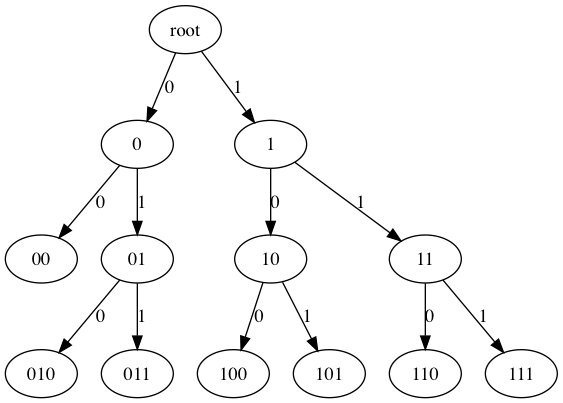
\includegraphics[width=0.5\textwidth]{./tree.png}
    % 设置标题
    \caption{码树示意图}
    % 设置图形引用名称
    \label{fig:tree}
  \end{figure}

\item 高效存取、序列化: 对树结点进行编码化之后,我们将树的存取转变成K-V存取,
  我们可以采用任意一种K-V存取引擎(如Tair、Redis等)对树结点进行存取。
  同时由于树是编码化的,我们可以很轻松的计算出任意结点的父亲、孩子、兄弟以及同层邻居结点等。
  考虑到效率问题,我们可以对结点进行批量存取,这一般依赖于下层的K-V存储引擎的设计,
  一般的K-V引擎都会提供这种批量存取功能。此外,我们还会对部分树结点进行cache,比如树上层的结点会被
  经常访问,并且所含结点数量较少,我们可以对这部分结点进行缓存,在二分类场景下,上层20层结点共有1M个结点,
  假设每个结点占用32byte,我们只需要32M内存就可以缓存这部分结点,从而避免远程加载。我们还对树设计掩码处理,
  以减少对不存在的结点访问。

\item 策略化采样: 采样将作为一个Tensorflow的Operation算子提供给用户使用,
  根据策略可以灵活执行不同的采样方法,采样策略可以配置,通过so动态库的形式加载运行,Operation的架构图如\ref{fig:op_arc}所示:
  \begin{figure}[!htbp]
    % 设置对齐格式
    \centering   %图片居于页面中部
    % 指定图形大小和图形名称
    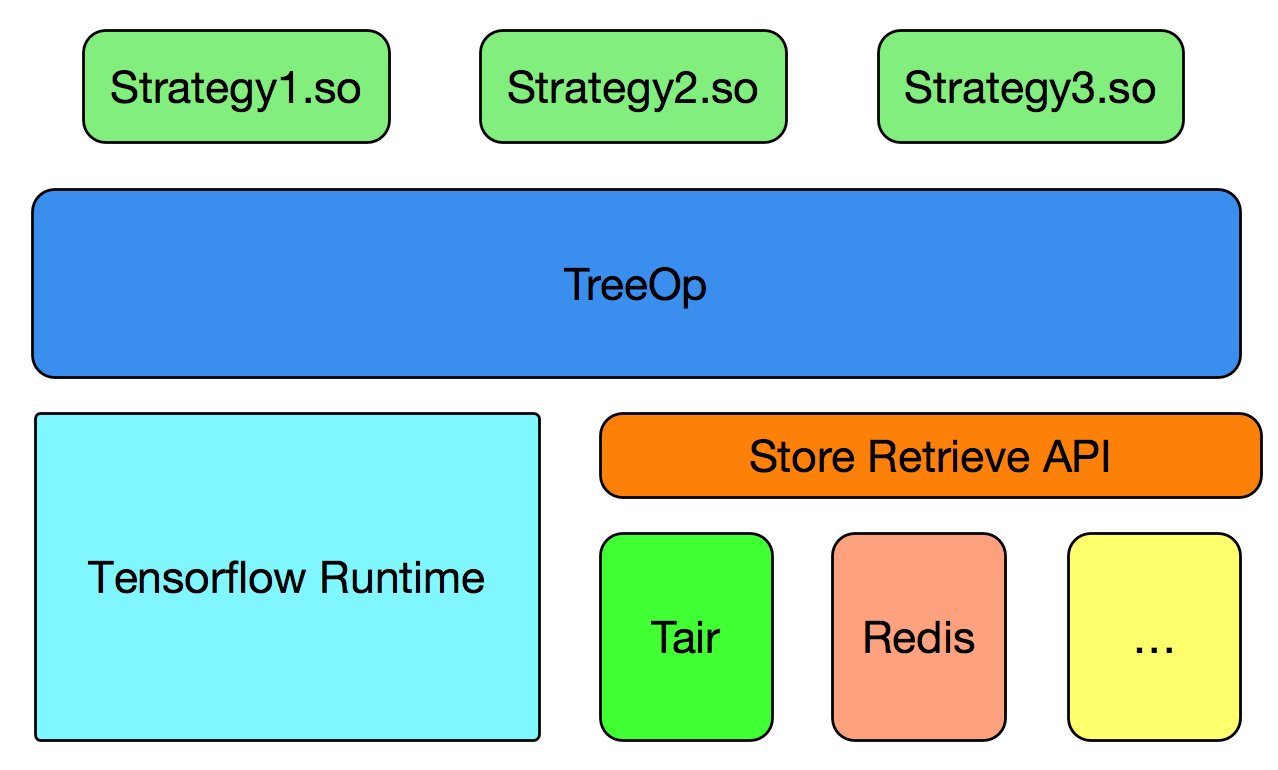
\includegraphics[width=0.75\textwidth]{./op_arc.png}
    % 设置标题
    \caption{Operation架构图}
    % 设置图形引用名称
    \label{fig:op_arc}
  \end{figure}

\item 层次化遍历: 编码后的树很容易计算出兄弟及邻居,从而很容易进行层次化遍历。
\end{enumerate}

\section{可能存在的风险}
\begin{enumerate}
\item 效率问题: 分布式存储后面临通信开销,需要尽可能的减少存取次数。
\item 更新: 未来在线系统可能有更新需求,更新需要考虑树结构的一致性。
\end{enumerate}

\section{排期}
待进一步讨论。

\section{总结}
通过将树结点进行编码,将树存储转换成分布式K-V存取,同时利用编码key的可计算性,K-V引擎的批量存取功能尽可能的降低分布式存取开销。
通过抽象采样接口,将采样实现和接口分离,实现采样的so注册加载,从而使得采样策略可以动态扩展及配置运行,加强了整个系统的灵活性。
经过前期验证,整个方案在技术上是可行的。
\end{document}